\documentclass[twocolumn,9pt]{jsproceedings}
\RequirePackage[l2tabu,orthodox]{nag}  % 古いコマンドやパッケージを使用した場合に警告する
%\usepackage{subcaption}
\usepackage[all,warning]{onlyamsmath}  % amsmath が提供しない数式環境を使用した場合に警告する
% \usepackage{flushend}  % 最終ページの2カラムの左右の高さを揃える
\usepackage{here} %図の場所の指定で[h](ここに貼る)を指定するためのパッケージ
\usepackage[dvipdfmx]{graphicx} %dvipdfmxはjpgやpngの張り込みのために使用
%\usepackage{graphicx}

% タイトル
\title{新卒だけどつくばチャレンジ出るよチームの\\つくばチャレンジ2024での取り組み}

\author{○池邉 龍宏\authorrefmark{1}、海老田 そら\authorrefmark{1}、春山 健太\authorrefmark{1}、大澤 来実\authorrefmark{1}\\森下 敢太\authorrefmark{1}、
深谷 和俊\authorrefmark{1}、藤江 謙伸\authorrefmark{1}、新宮 義規\authorrefmark{1}}

\etitle{Our Team's Efforts in Tsukuba Challenge 2024 as New Graduate Participants}

\eauthor{○Tatsuhiro IKEBE\eauthorrefmark{1}、Sora EBITA\eauthorrefmark{1}、Kenta HARUYAMA\eauthorrefmark{1}、Kurumi OSAWA\eauthorrefmark{1}\\Kanta MORISHITA\eauthorrefmark{1}
Kazutoshi FUKAYA\eauthorrefmark{1}、Kenshin FUJIE\eauthorrefmark{1}、Yoshiki SHINGU\eauthorrefmark{1}}

\affiliation{新卒だけどつくばチャレンジ出るよ}

\begin{document}
\maketitle

\authorreftext{1}{社会人}
\eauthorreftext{1}{Working adult}

% 本文
\section{緒言}\label{sec:1}

「新卒だけどつくばチャレンジ出るよ」チームは、
同じ会社内でつくばチャレンジへの参加を希望するメンバーが集まって結成されたチームである。
チームメンバーは2024年入社の新規学卒者(以下、新卒)8名で構成されており、
つくばチャレンジの参加経験は初参加の者から複数年の経験者まで様々である。

本チームの参加目的は、新卒であってもつくばチャレンジに参加できることを証明することである。
また、本チームの活動を通じて、来年度以降、新卒での参加チームが増えることを目指している。
この目的を達成するため、本チームでは以下の目標を設定した。
\begin{itemize}
  \item[1] 参加登録
  \item[2] 独自設計したロボットによる車検合格
  \item[3] ロボットに搭載されたセンサから得られる情報から歪みの無い地図を取得
  \item[4] 確認走行区間を完走
\end{itemize}


本稿では、これらの目標に対する取り組みとその結果について述べる。
本稿の構成は次の通りである。
1章では、参加メンバーおよび本チームの参加目的・目標について説明する。
2章ではロボットのハードウェアおよびソフトウェアの構成について述べ、
3章では本走行の結果と明らかになった課題を示す。
4章では、本年度のつくばチャレンジでは活用しなかったものの、本チームで取り組んだ内容を紹介し、
最後に5章で結言を述べる。

\section{ロボットの構成}

\subsection{概要}
本チームでは、新卒がつくばチャレンジに参加しやすい環境を整えるため、
できるだけ安価に作成可能なロボット構成を目指し、ハードウェア設計および部品選定を行った。
\ref{sub:hardware} 節では、採用したロボットプラットフォーム、センサ、ロボット保護カバーなどの詳細について説明する。

ソフトウェアに関しては、本チームは ROS 2 \cite{ROS 2} を基盤として構築した。
ソフトウェアの特徴については、\ref{sub:software} 節以降で述べる。


\subsection{ハードウェア構成}\label{sub:hardware}
ロボットの外観を図\ref{fig:trainee}に示す。
本ロボットは、ODrive社製の既製品である、BotWheel Explorer Kit\cite{odrive}がベースになっている。

\begin{figure}[h]
  \begin{center}
    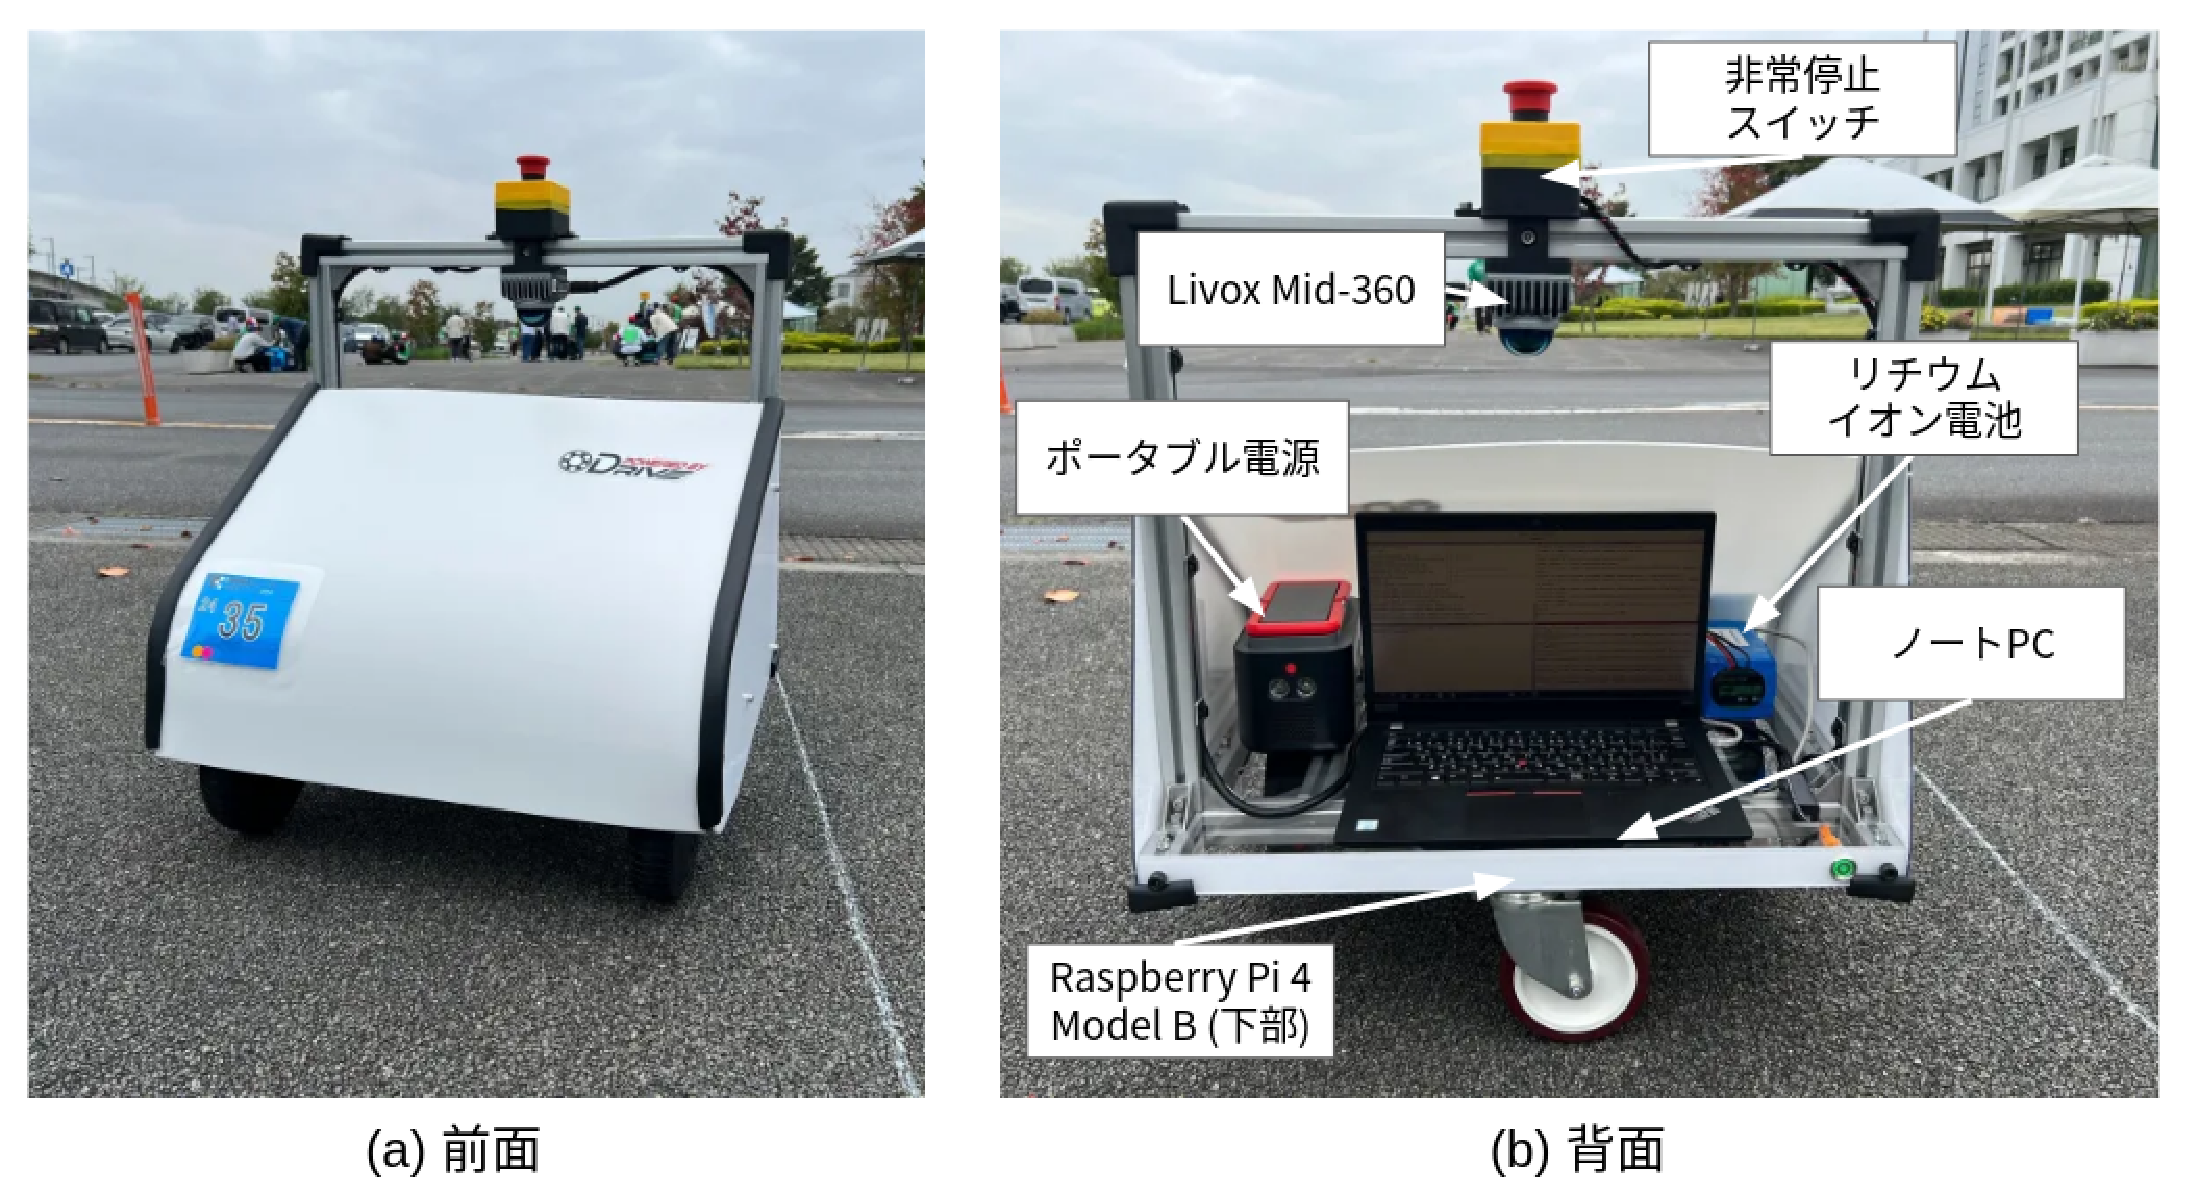
\includegraphics[width=1.0\linewidth]{figs/trainee.pdf}
    \caption{チームの機体(機体名: トレーニー)}
    \label{fig:trainee}
  \end{center}
\end{figure}

\begin{figure}[h]
  \begin{center}
    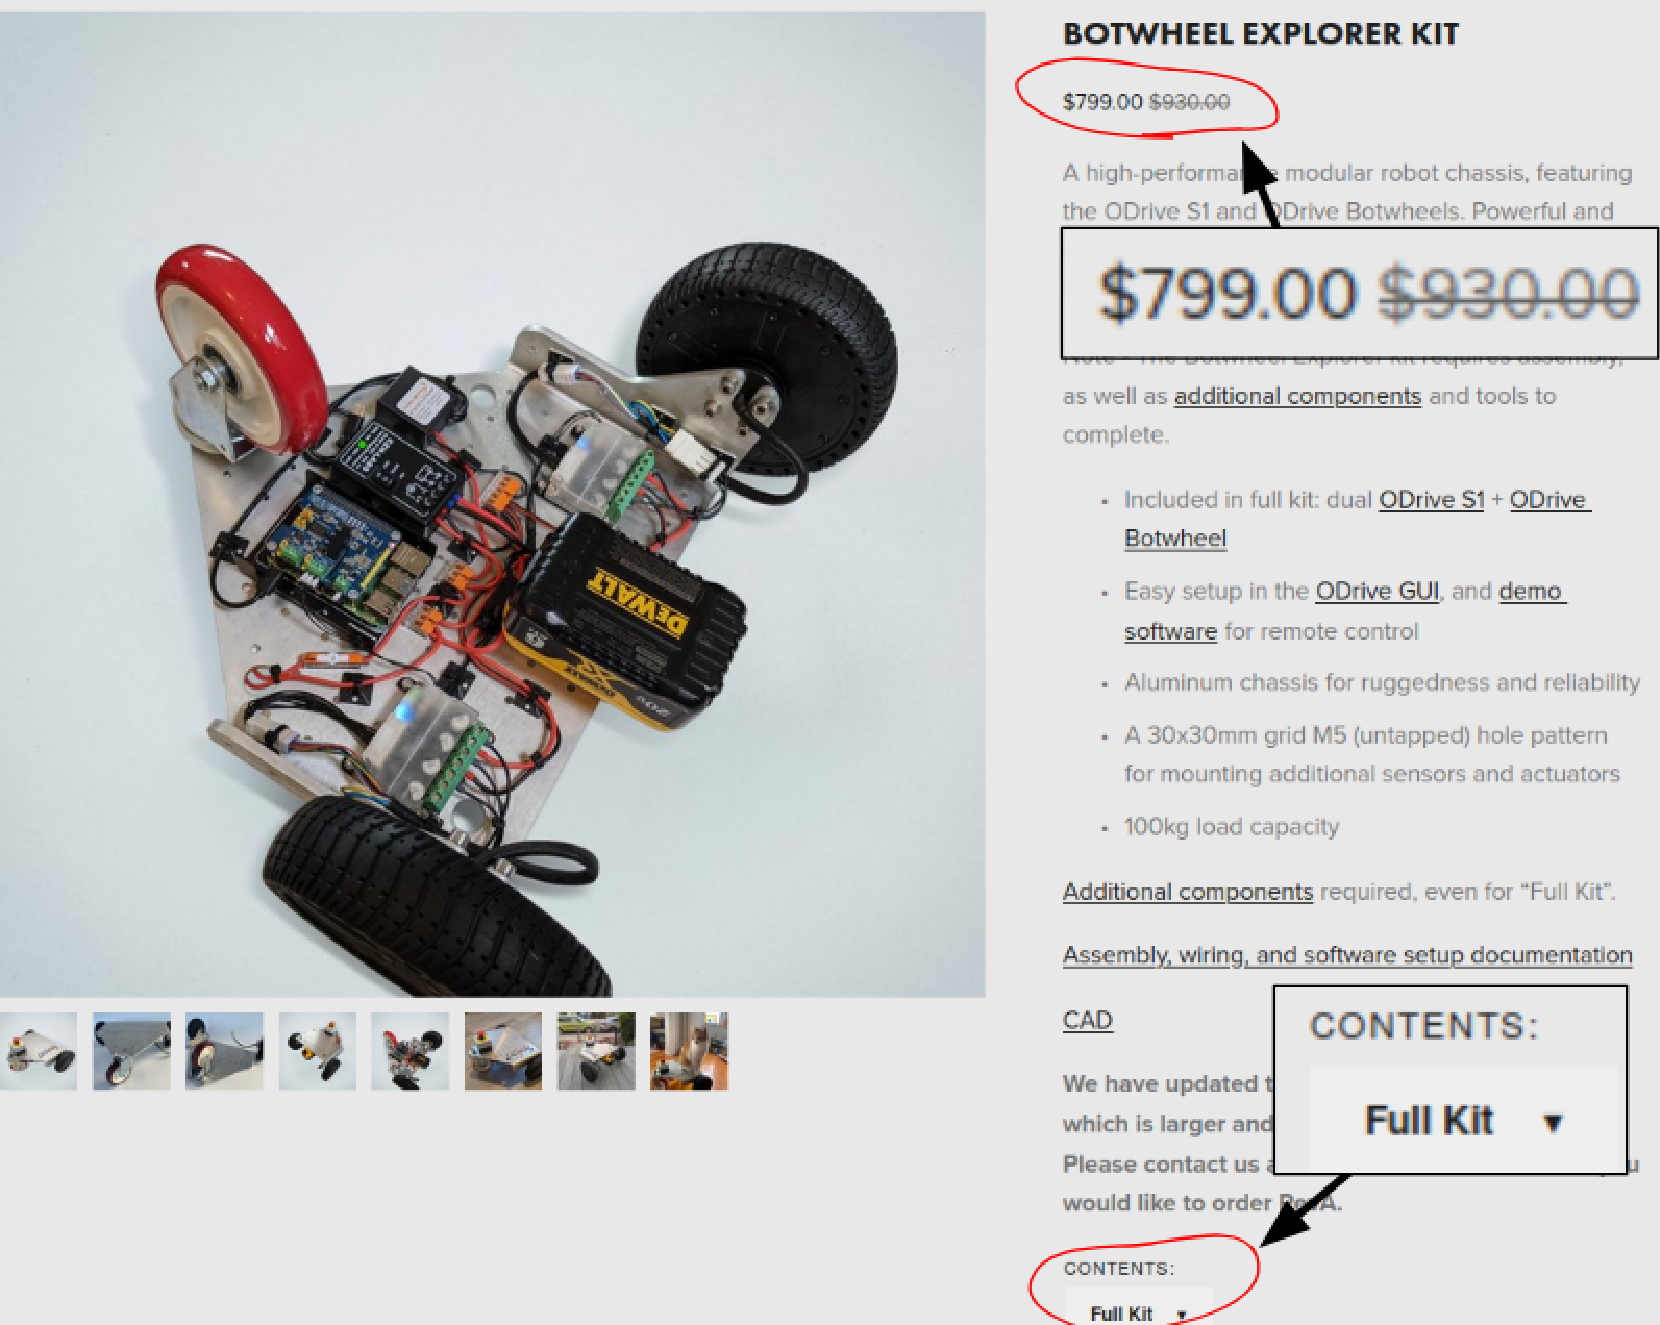
\includegraphics[width=0.8\linewidth]{figs/b_kit_price.pdf}
    \caption{BotWheel Explorer Kitの金額および内容について}
    \label{fig:b_robot_price}
  \end{center}
\end{figure}

本ロボットをベースとして採用した最大の理由は、価格の安さである。
図\ref{fig:b_robot_price}の通り、BotWheel Explorer Kitは799ドルで購入可能であり、
同様の構成を持つ他のロボットと比較しても圧倒的に安価である。
さらに、「Full Kit」として販売されており、一通りの部品が揃っている点も魅力的である。
そのため、本チームはこのキットを採用することにした。

しかし、「Full Kit」といっても電装部品が全て含まれているわけではない。
商品ページの画像からは、全ての部品が揃っているように見えるが、
実際には不足している部品もあるため、購入時には注意が必要である。
また、購入時には円相場や海外手数料も考慮する必要がある。

「Full Kit」に含まれる部品の一覧を表\ref{tab:botwheel_kit}に示す。
このキットには、駆動用のインホイールモータ、制御用のモータドライバ、
モータ取り付け用のシャーシ、モータドライバとインホイールモータ間の通信に必要なCANハーネスなどが含まれている。
\begin{table}[h]
  \centering
  \caption{BotWheel Explorer Kit の部品一覧}
  \begin{tabular}{|l|c|l|}
      \hline
      \multicolumn{3}{|c|}{\textbf{BotWheel Explorer Kit(Full Kit)}} \\
      \hline
      部品 & 数量 & 詳細 \\
      \hline
      ODrive S1 & 2 & モータドライバー \\
      ODrive Botwheel & 2 & インホイールモータ \\
      Chassis Plate & 1 & シャーシ \\
      Caster & 1 & キャスター \\
      CAN harnesses & 2 & CANハーネス \\
      \hline
  \end{tabular}
  \label{tab:botwheel_kit}
\end{table}


BotWheel Explorer Kitは、前方に2つの駆動輪、後方に1つの受動輪を備え、三角形のシャーシに取り付けられたシンプルな足回りのみのユニットである。
しかし、標準の状態では保護カバーがなく、雨や外部環境の影響を受けやすい。
そのため、本チームでは、図\ref{fig:trainee_flame}(a)のように20×20mmのアルミフレームをシャーシに固定し、
(b)に示すようにポリプレートのカバーを取り付けることで、耐環境性を向上させた\cite{PE960_1}。

ポリプレートは厚さ3mmの素材であり、手で簡単に曲げられるため、曲面を持つ保護カバーの作成が容易である。
さらに、シャーシにはナットが飛び出している箇所が多く、平坦なスペースが限られていた。
そのため、アルミフレームの上部にポリカーボネートの板を取り付け、ノートPCやバッテリーを搭載できるスペースを確保した。

% また、つくばチャレンジの規定ではロボットの最低高さを600mm以上とする制約がある。
また、つくばチャレンジの規定ではロボットの全高を0.6m以上とする制約がある。
さらに、運搬の利便性を考慮し、アルミフレームを上部に伸ばして台車の持ち手のような構造とした。
非常停止スイッチおよび3次元LiDARは、3Dプリンタで製作した治具を用い、機体上部の高さ750mmのアルミフレームに固定した。

アルミフレームや治具の設計には Fusion 360 \cite{Fusion360} を使用した。
しかし、無料ライセンスではチーム開発ができなかったため、CADモデルの共有には Onshape \cite{Onshape} を用いた。


センサ構成について、図\ref{fig:botwheel-explorer-schematic}に示す。
\begin{figure}[h]
  \begin{center}
    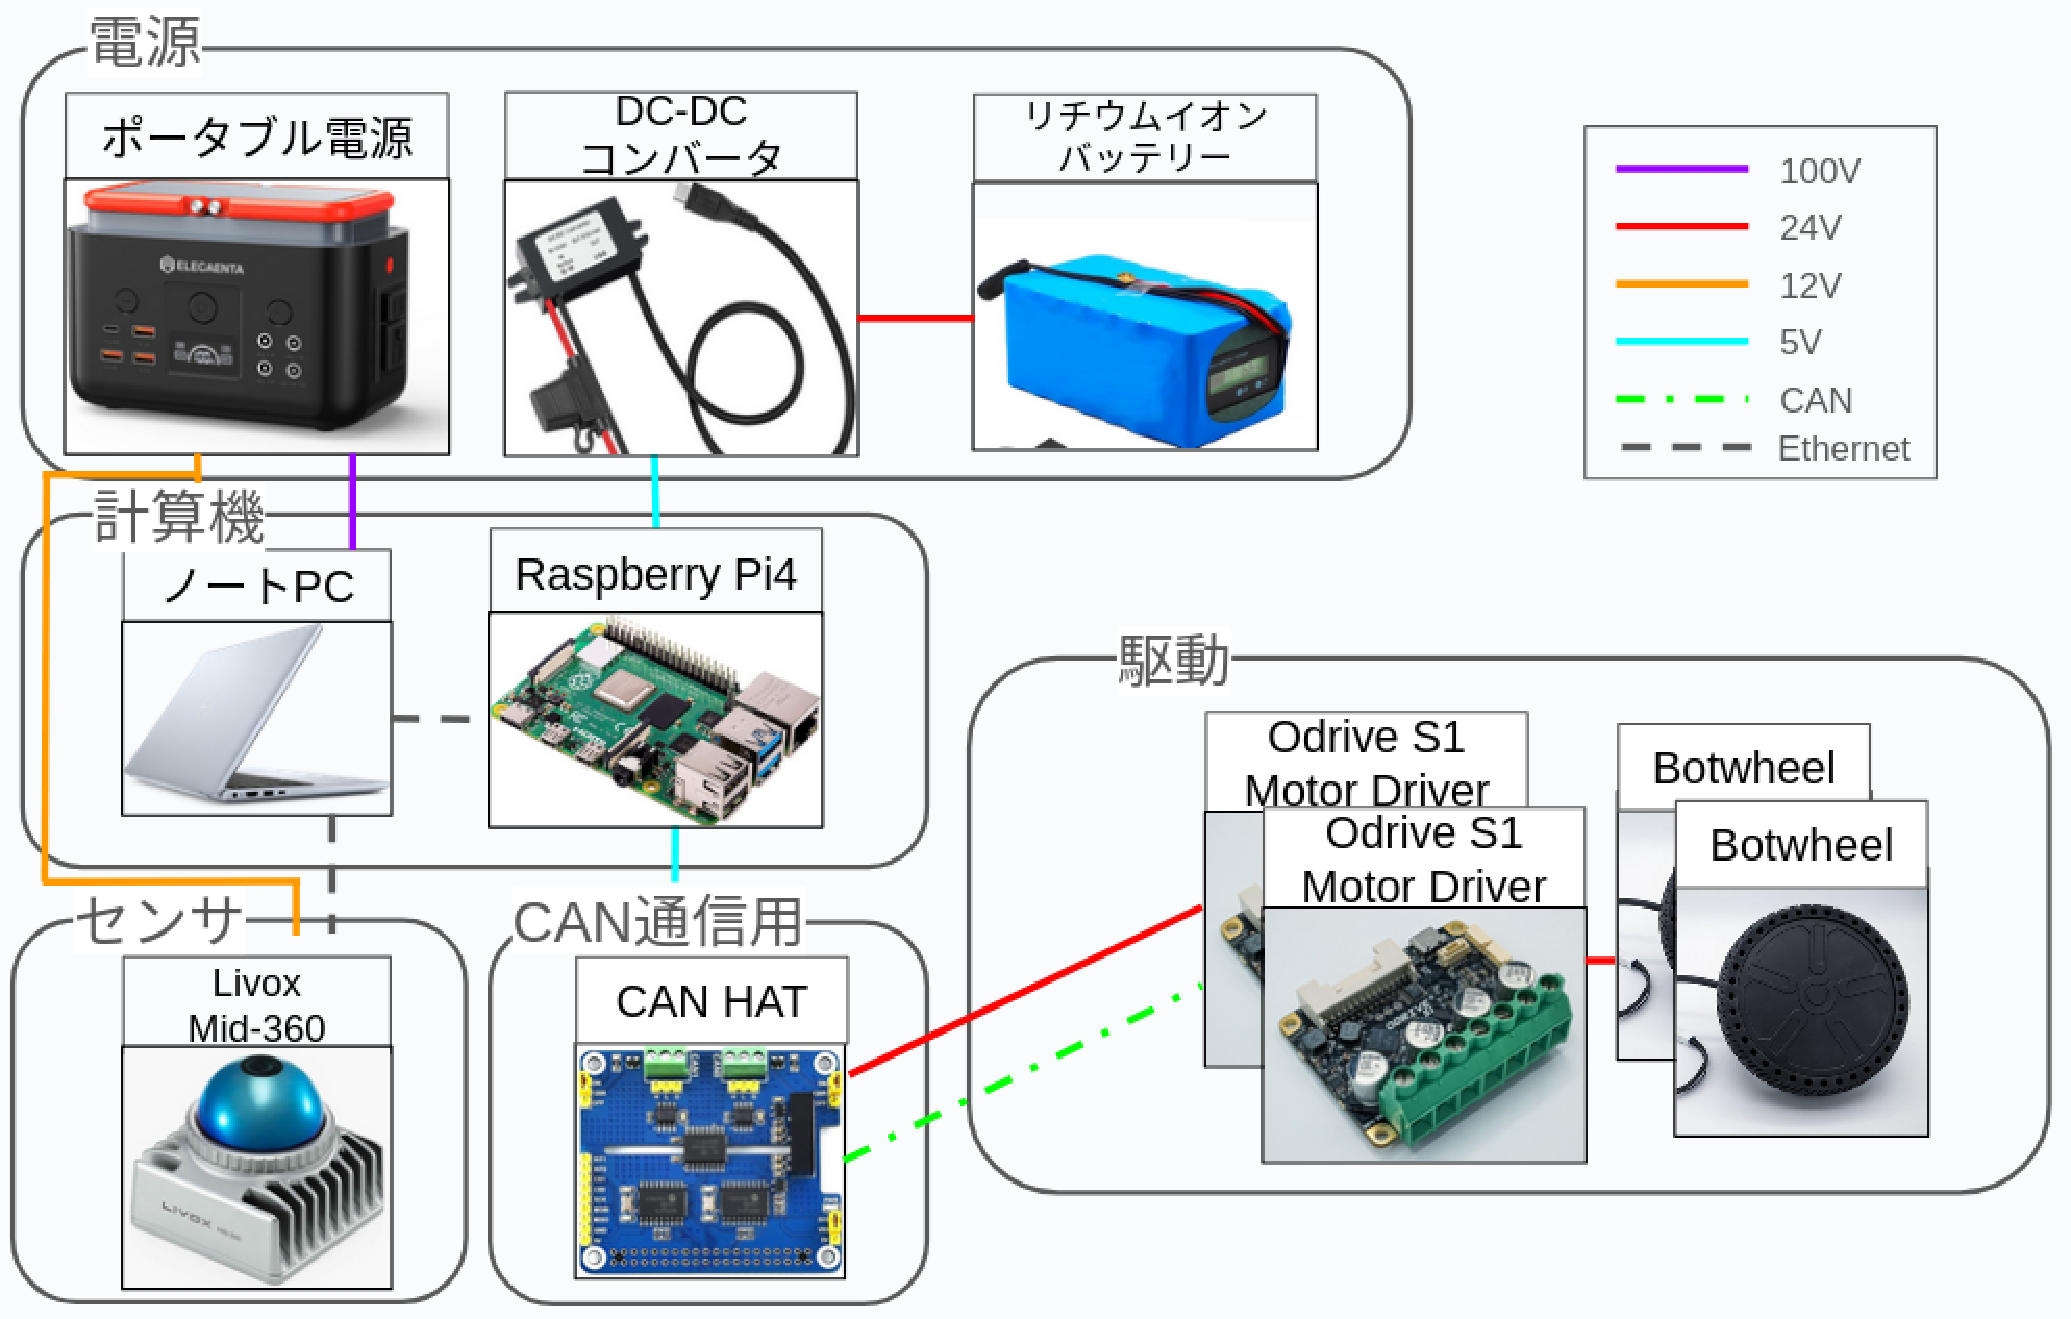
\includegraphics[width=1.0\linewidth]{figs/botwheel-explorer-schematic.pdf}
    \caption{機体の回路構成}
    \label{fig:botwheel-explorer-schematic}
  \end{center}
\end{figure}

\begin{figure}[h]
  \begin{center}
    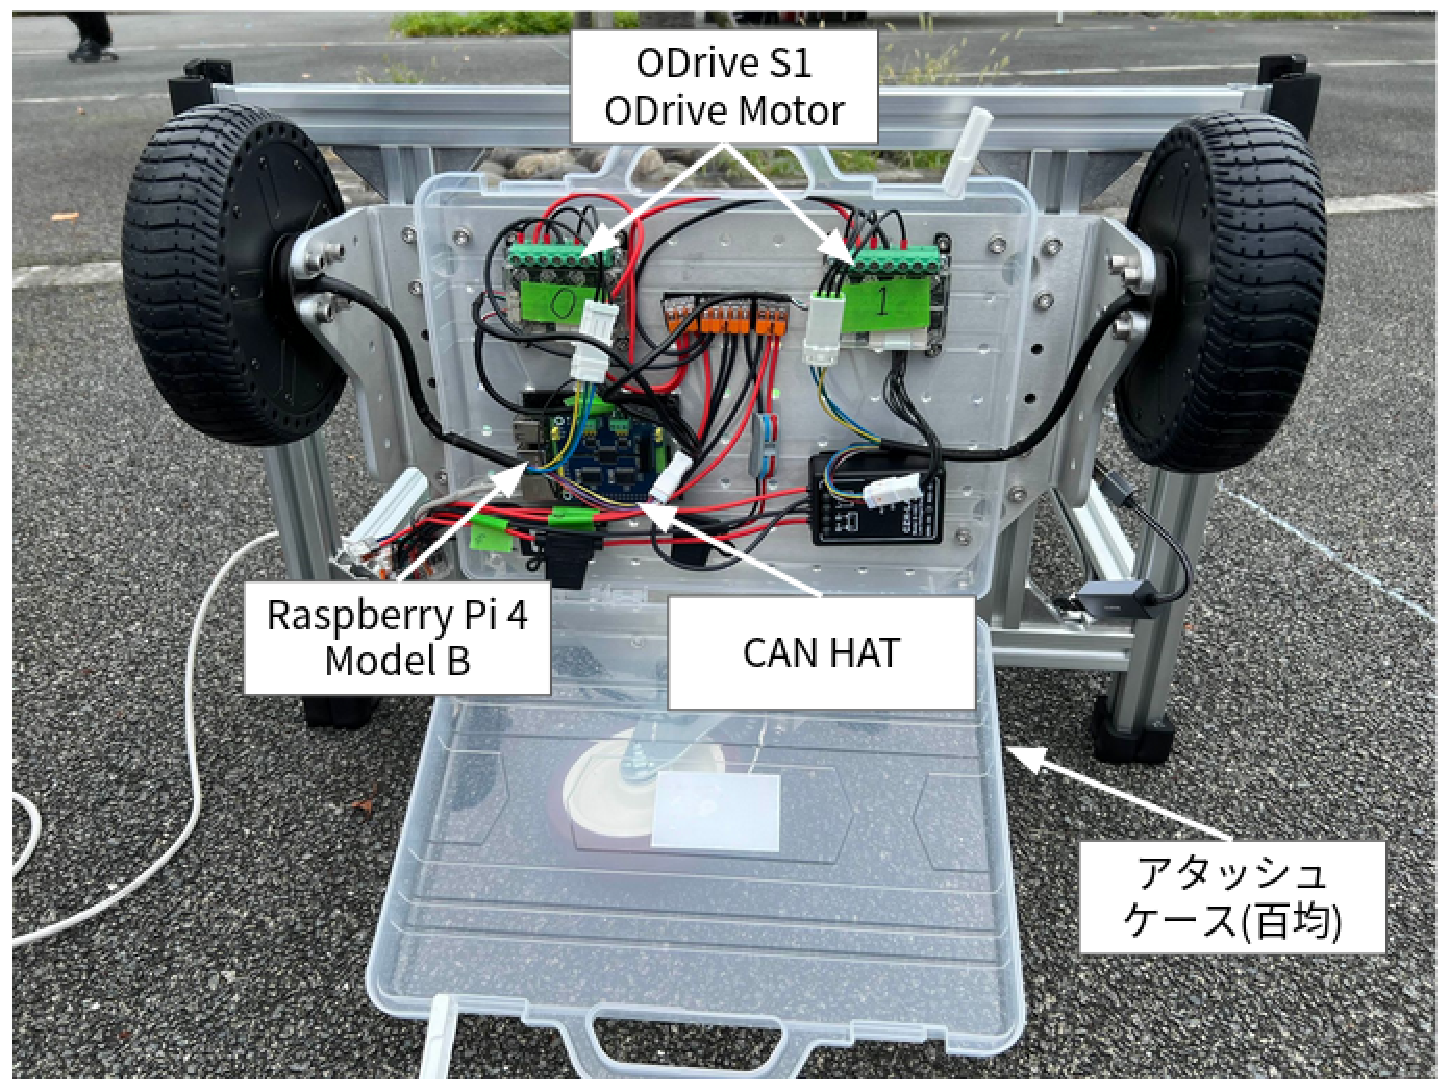
\includegraphics[width=1.0\linewidth]{figs/trainee_under.pdf}
    \caption{機体の回路構成(実機)}
    \label{fig:trainee_under}
  \end{center}
\end{figure}

センサとしては、Livox社製のMid-360\cite{mid360}を搭載した。
Mid-360を採用した理由は以下の4点である。

\begin{itemize}
  \item[1] 本走行エリアでの使用を想定した際に、測定可能な距離が 40〜70 m と十分に長いこと
  \item[2] 1台のLiDARで360度の測定が可能であること
  \item[3] 1台10万円と、安価であること
  \item[4] IMUが内蔵されていること
\end{itemize}

Mid-360の取り付け位置は、自己位置推定と障害物回避の両立を目指して設計した。
自己位置推定では、植木などのランドマークを検知しながら、地面の勾配の影響を受けないようにするため、
地面から高さ10〜30 cmの3次元点群を2次元に変換して使用する。
一方で、障害物回避では、地面周辺の死角を最小限に抑えることが求められる。
そのため、機体を覆うカバーによる死角を考慮しつつ、最適なLiDARの取り付け位置を検討した。
具体的には、図\ref{fig:lidar_pos}に示すようにOnshapeの3Dスケッチ機能を用いてカバーによる死角を可視化し、
最も死角が少なくなる取り付け位置を算出した。
その結果、図\ref{fig:trainee_flame}(b)に示すような位置に
LiDARを下向きに取り付けることで、自己位置推定と障害物回避の両方に適したセンサ配置を実現した。

\begin{figure}[h]
  \begin{center}
    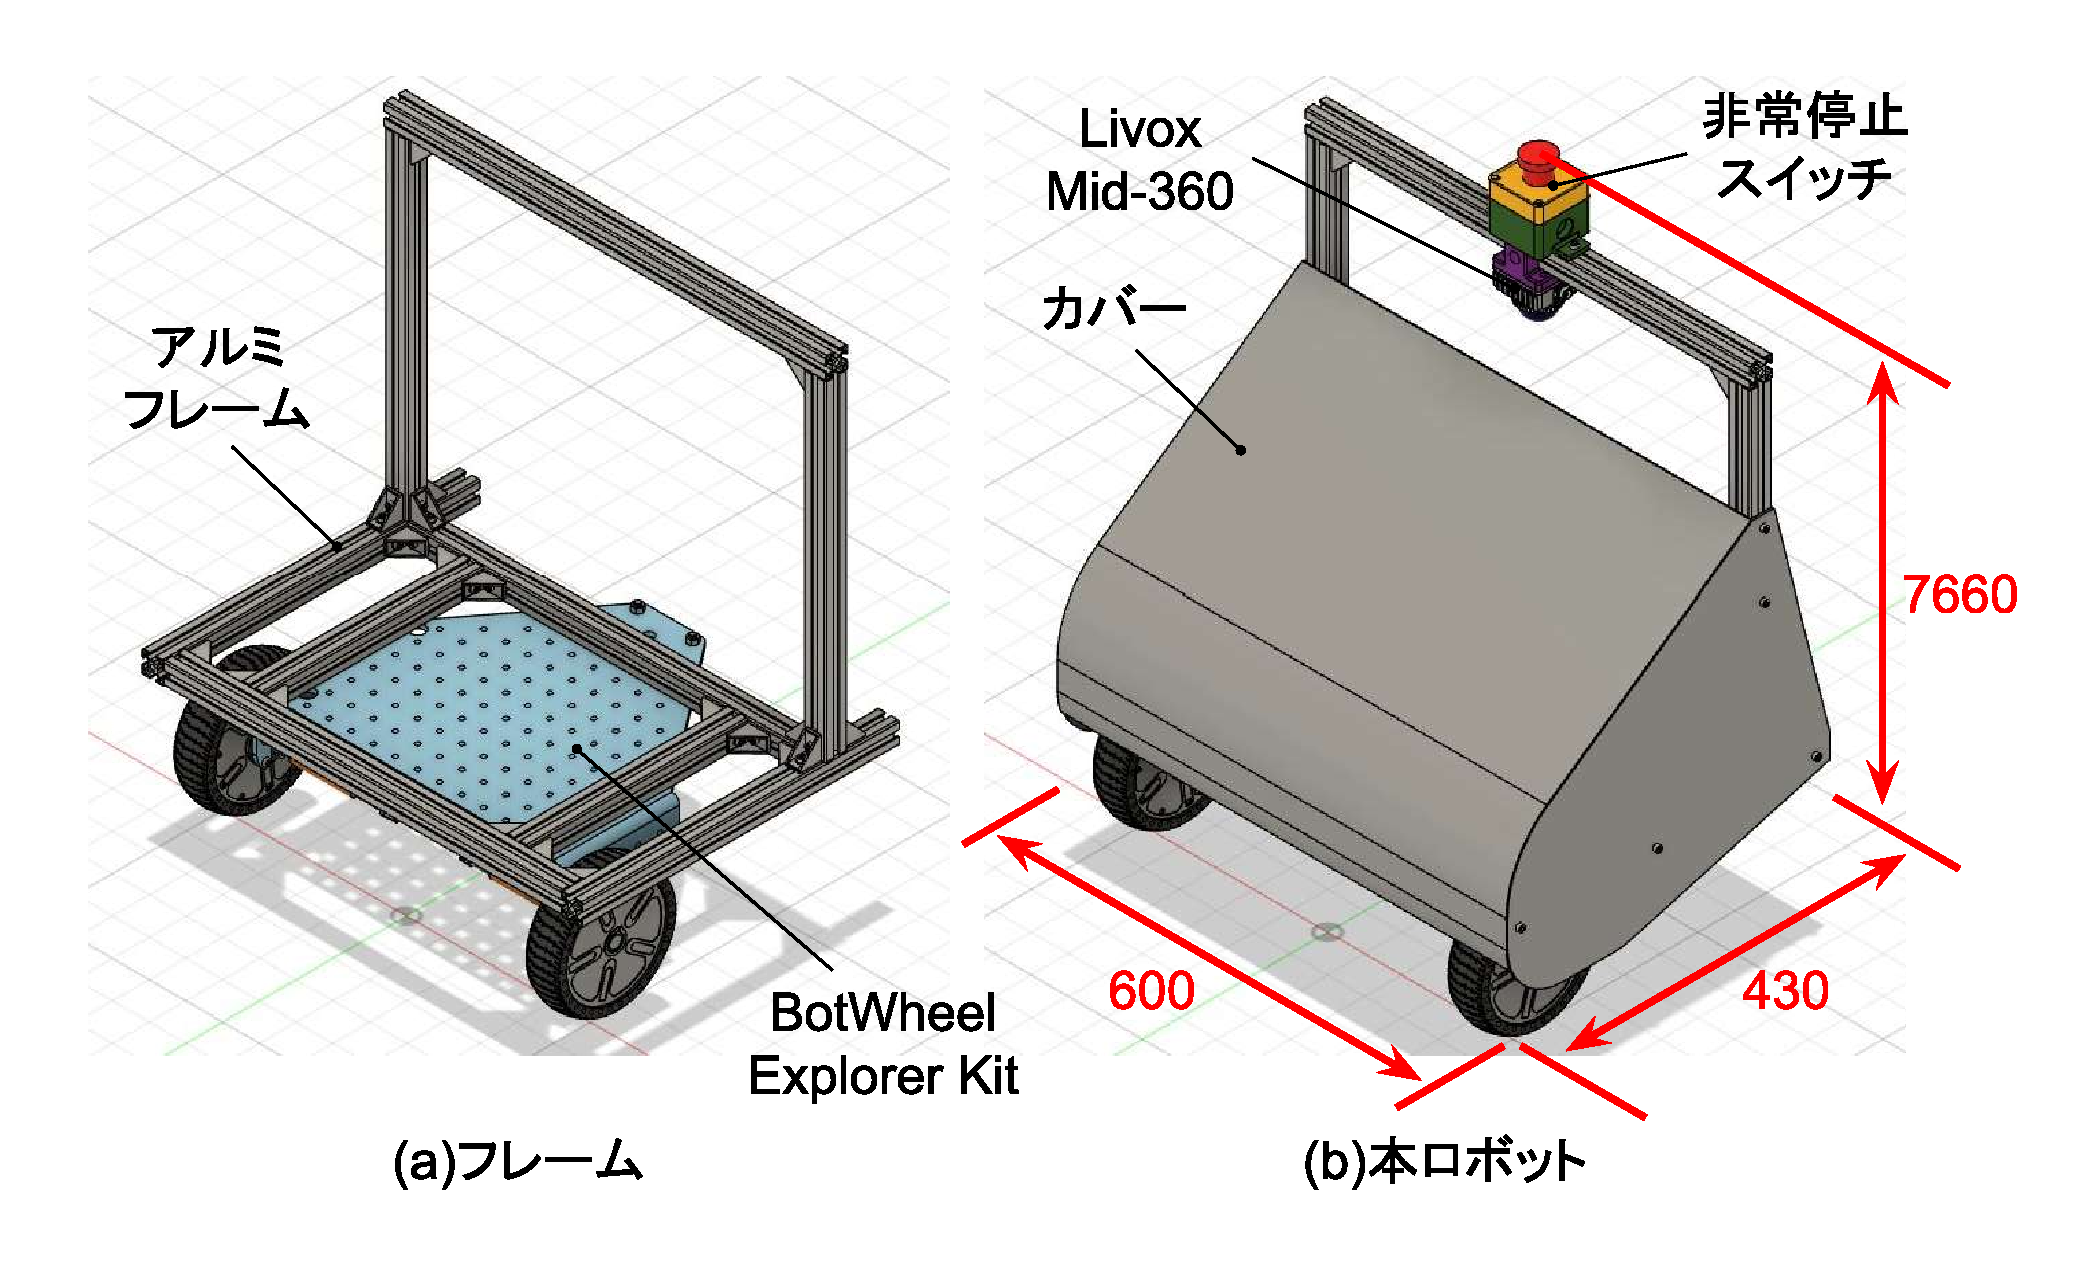
\includegraphics[width=1.0\linewidth]{figs/robot_flame.pdf}
    \caption{ハードウェア設計}
    \label{fig:trainee_flame}
  \end{center}
\end{figure}

\begin{figure}[h]
  \begin{center}
    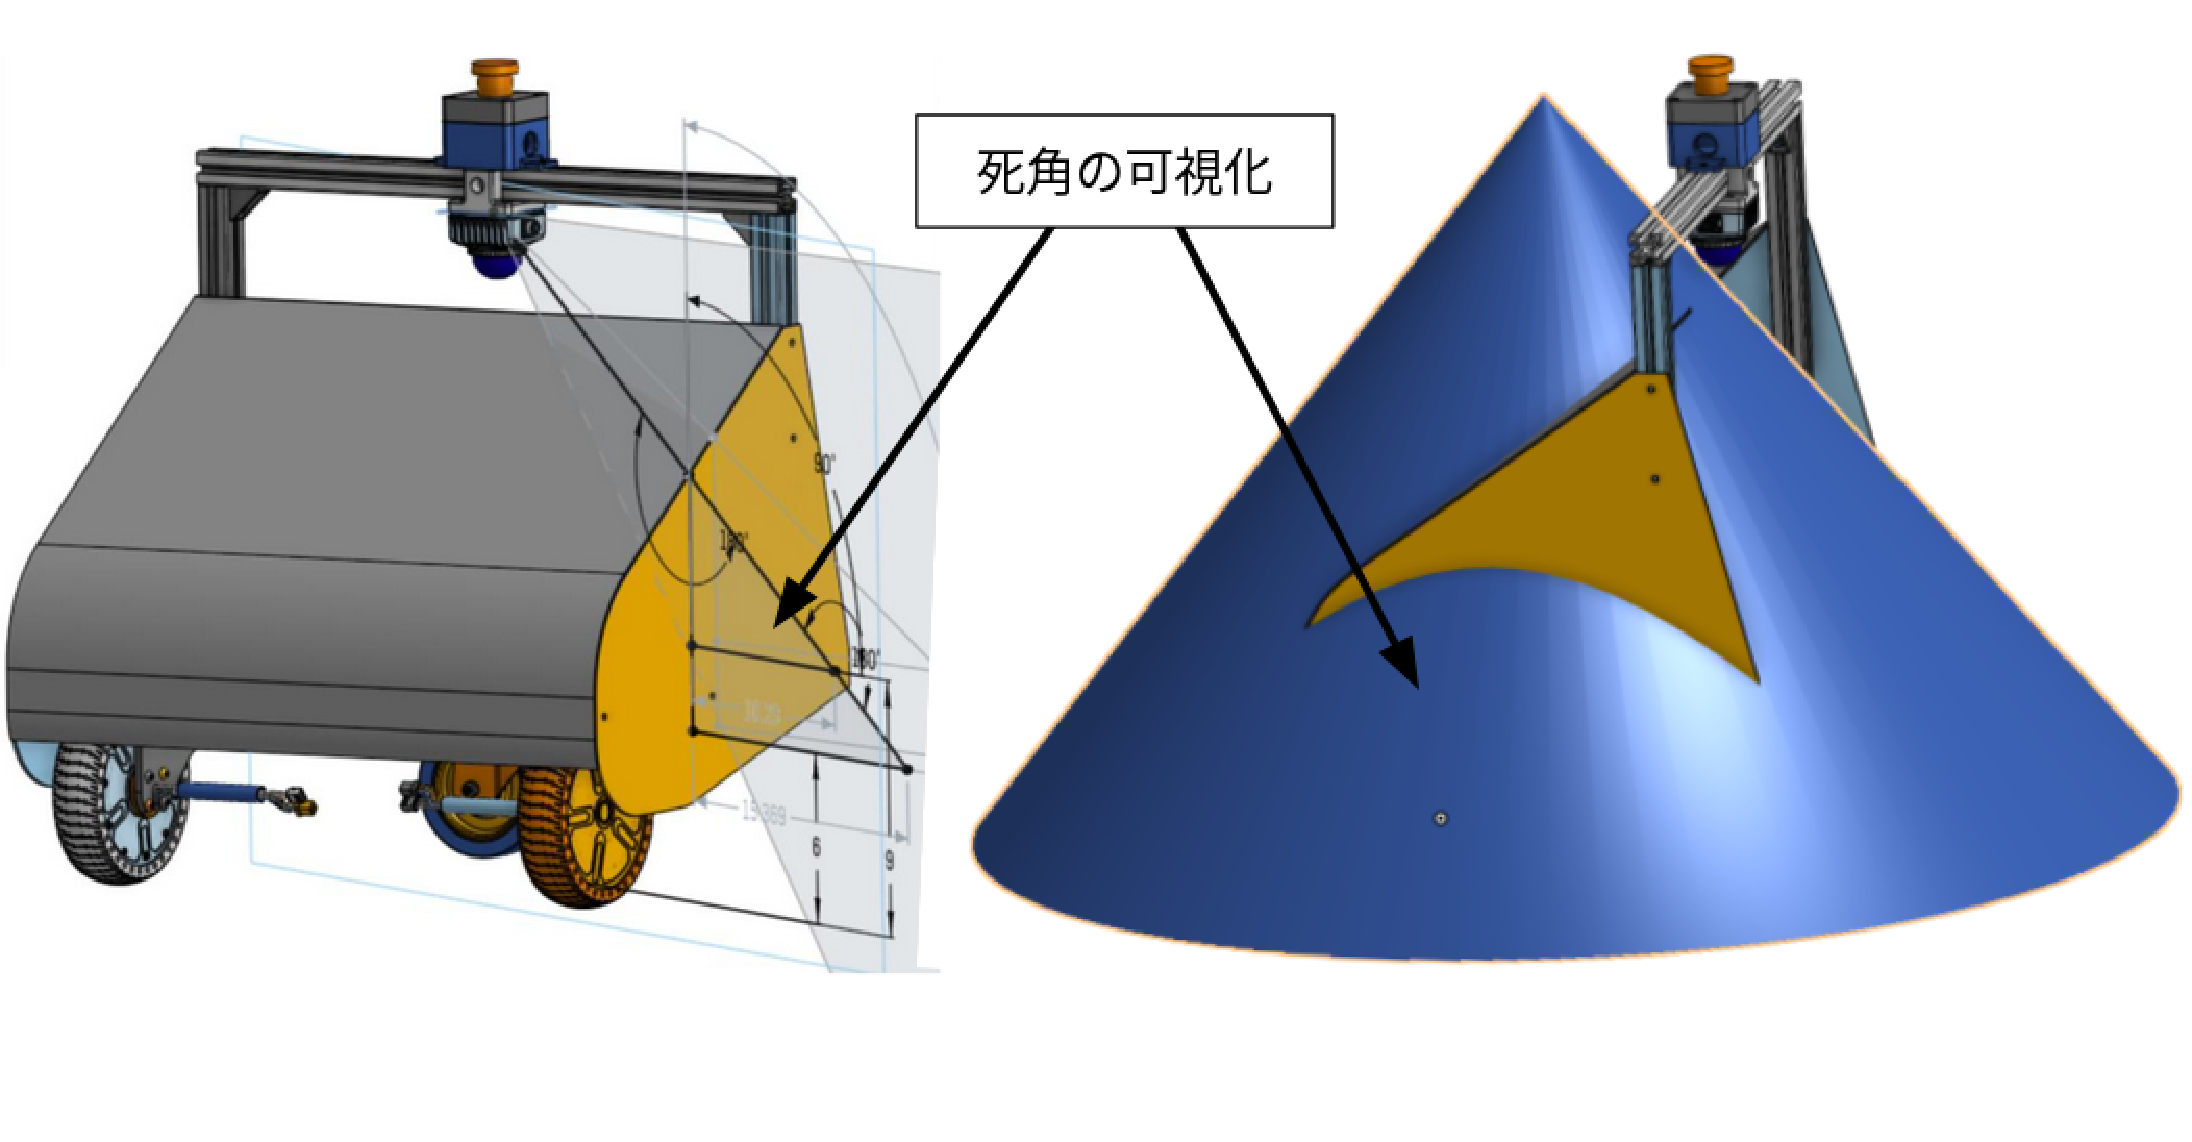
\includegraphics[width=1.0\linewidth]{figs/lidar_position_onshape.pdf}
    \caption{LiDARの死角の可視化}
    \label{fig:lidar_pos}
  \end{center}
\end{figure}

\subsection{ソフトウェア構成}\label{sub:software}

本チームで使用したソフトウェアは、すべて Ubuntu 22.04 上で動作し、自作パッケージと既存の ROS 2 Humble 用パッケージを活用した。
これらのパッケージは GitHub 上で公開されており、誰でも利用可能である。
また、ソフトウェア開発環境をチーム内で統一するため、Docker 上に ROS 2 Humble 環境を構築した。

本チームのシステム構成を図 \ref{fig:shinsotu_system_diagram} に示す。
ロボットに搭載された 3次元LiDAR は、センサ情報(点群・IMU)を Ethernet を介してノート PC に送信する。
ノート PC は、自己位置推定・経路生成・経路追従などの主要な計算を担当する。
ノートPCの諸元を表\ref{table:laptop}に示す. 
計算結果に基づく制御指令は、Ethernet を介して Raspberry Pi 4B に送信され、
Raspberry Pi 4B に接続された CAN HAT から ODrive S1 を介して CAN 通信を行い、機体を制御する。

\begin{table}[H]
  \centering
  \caption{ノートPCの諸元}
  \label{table:laptop}
	  \begin{tabular}{|l|p{1.0cm}|l|}
    \hline
    CPU & RAM\\ 
    \hline
    第13世代 インテル® Core™ i5プロセッサー 1334U  & 16GB \\ 
    \hline
  \end{tabular}
\end{table}

\begin{figure}[h]
  \begin{center}
    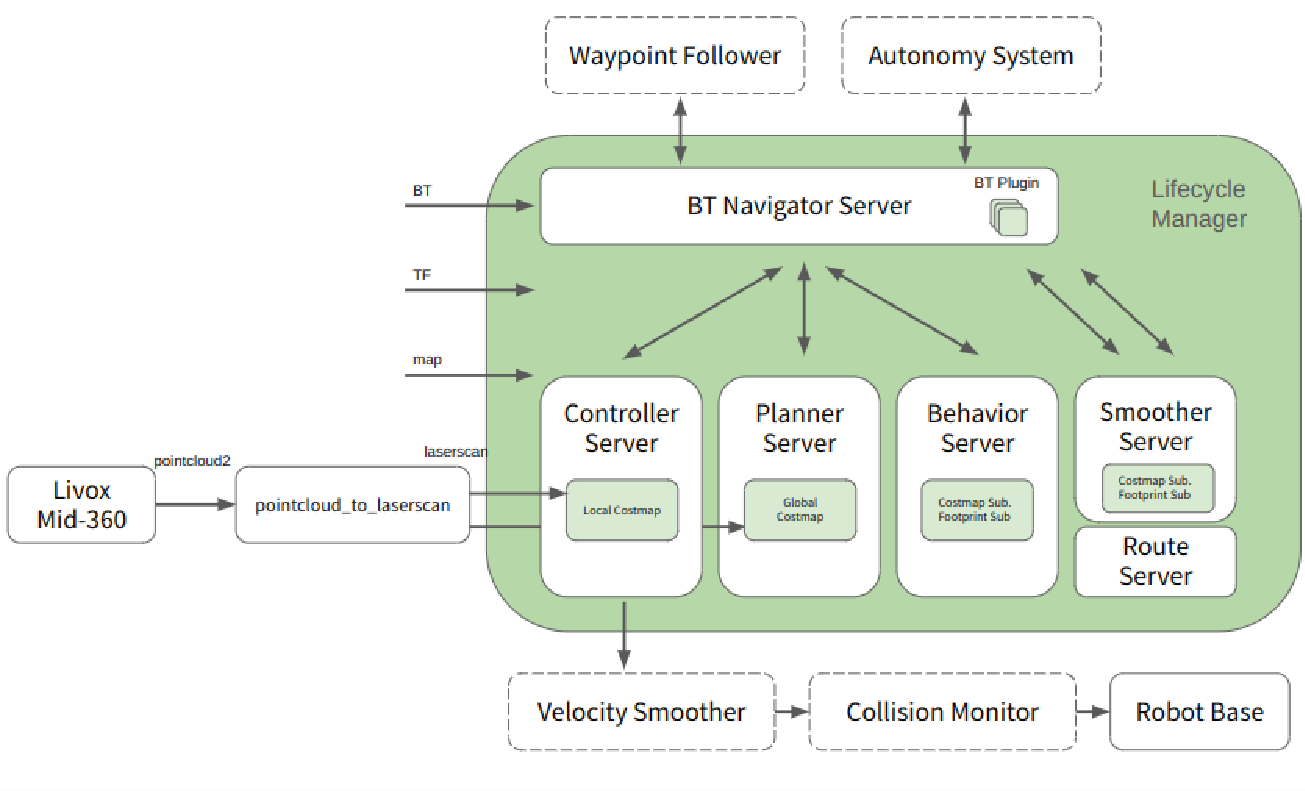
\includegraphics[width=1.0\linewidth]{figs/shinsotu_system_diagram.pdf}
    \caption{システム構成 \cite{nav2_docs}}
    \label{fig:shinsotu_system_diagram}
  \end{center}
\end{figure}

自律移動の手法として、3次元LiDAR で取得したスキャンデータから事前に作成した 2 次元の環境地図と、
走行中に取得するスキャンデータとのマッチングに基づいて自己位置推定し、自律走行する方式を採用した。
2 次元地図の作成には 2 次元のレーザースキャン情報が必要となるが、
使用した LiDAR は 3 次元点群を出力するため、3 次元点群を 2 次元に変換する処理を行った。
この変換には、pointcloud\_to\_laserscan \cite{pcl_lsc} を使用した。

自己位置推定には、navigation2 の自己位置推定パッケージ nav2\_amcl \cite{nav2_amcl} を使用した。
経路計画と障害物回避には Nav2 \cite{nav2} を採用し、経路計画は 2 次元環境地図上で実行された。計画は、推定されたロボットの姿勢情報を基に算出される。
また、2 次元環境地図の作成には slam\_toolbox \cite{slam_toolbox} を使用した。

nav2\_amcl による自己位置推定の不確実性を低減する手法として、ロボットの姿勢情報と IMU の情報をカルマンフィルタで統合する方法がある。
しかし、本チームでは実装が間に合わなかったため、IMU の情報は使用しなかった。

\section{本走行・実験走行の結果}
\subsection{本走行の結果}

つくばチャレンジ2024での本走行の結果を表\ref{MainRun}に示す。
本走行の結果は 表 に示す通り、429m となった。
動画 \cite{youtube_real_run} のように、走行中にアクシデントは発生せず、終始スムーズに自律走行をすることができた。
本チームの目標である 確認走行区間の完走は達成できたが、
この目標に注力した結果、それ以降の区間の地図作成が間に合わず、本走行の継続はできなかった。
\begin{table}[H]
  \caption{本走行の結果の詳細}
  \label{MainRun}
  \begin{tabular}{|c|c|p{4.0cm}|}
    \hline
    走行距離 & リタイアの理由 \\
    \hline
    429m   & 確認走行区間以降の地図が未取得であったため \\
    \hline
  \end{tabular}
\end{table}

\subsection{本チームの目標の達成度}

\ref{sec:1}章 で説明した本チームの目標について、達成度を評価する。
各目標は、実現可能であると考えた上で設定したものである。

\paragraph{参加登録}
参加登録については、特に困難な点はなく、問題なく目標を達成した。
本チームのメンバーは、つくばチャレンジへの参加に意欲的なメンバーを募ったため、登録に関して意見の対立なども生じなかった。
必要だったのは、仕事と並行しながら限られた時間で進捗を生み出す覚悟であった。

\paragraph{独自設計したロボットでの車検合格}
独自設計したロボットによる車検合格についても、問題なく目標を達成した。
本チームは、図\ref{fig:trainee_flame}のように
BotWheel Explorer Kitをベースに機体を独自設計し、
図\ref{fig:trainee}に示す機体を作成した。
機体の設計においては、車検のポイントとなる以下の項目を重点的に考慮した。
\begin{itemize}
  \item 車輪の露出防止
  \item 配線の適切な取り回し
  \item 機体の全高
  \item 角張った部分の保護
  \item 非常停止スイッチの押しやすさ
\end{itemize}


\paragraph{ロボットに搭載されたセンサから得られる情報から歪みの無い地図を取得}

ロボットに搭載されたセンサ情報を用いた歪みのない地図の取得についても、問題なく目標を達成した。
Mid-360 の照射パターンは、他の 3 次元 LiDAR と異なり、各スキャンごとに同じ位置を計測するわけではないため、特殊であり、
歪みを抑えた地図を作成できるかどうかの見通しは立っていなかった。
しかし、pointcloud\_to\_laserscan と slam\_toolbox を使用したところ、予想に反して容易に地図を生成できた。
その結果、図 \ref{fig:map} に示すように、実環境と比較してもほぼ歪みのない地図が得られた。

\begin{figure}[h]
  \begin{center}
    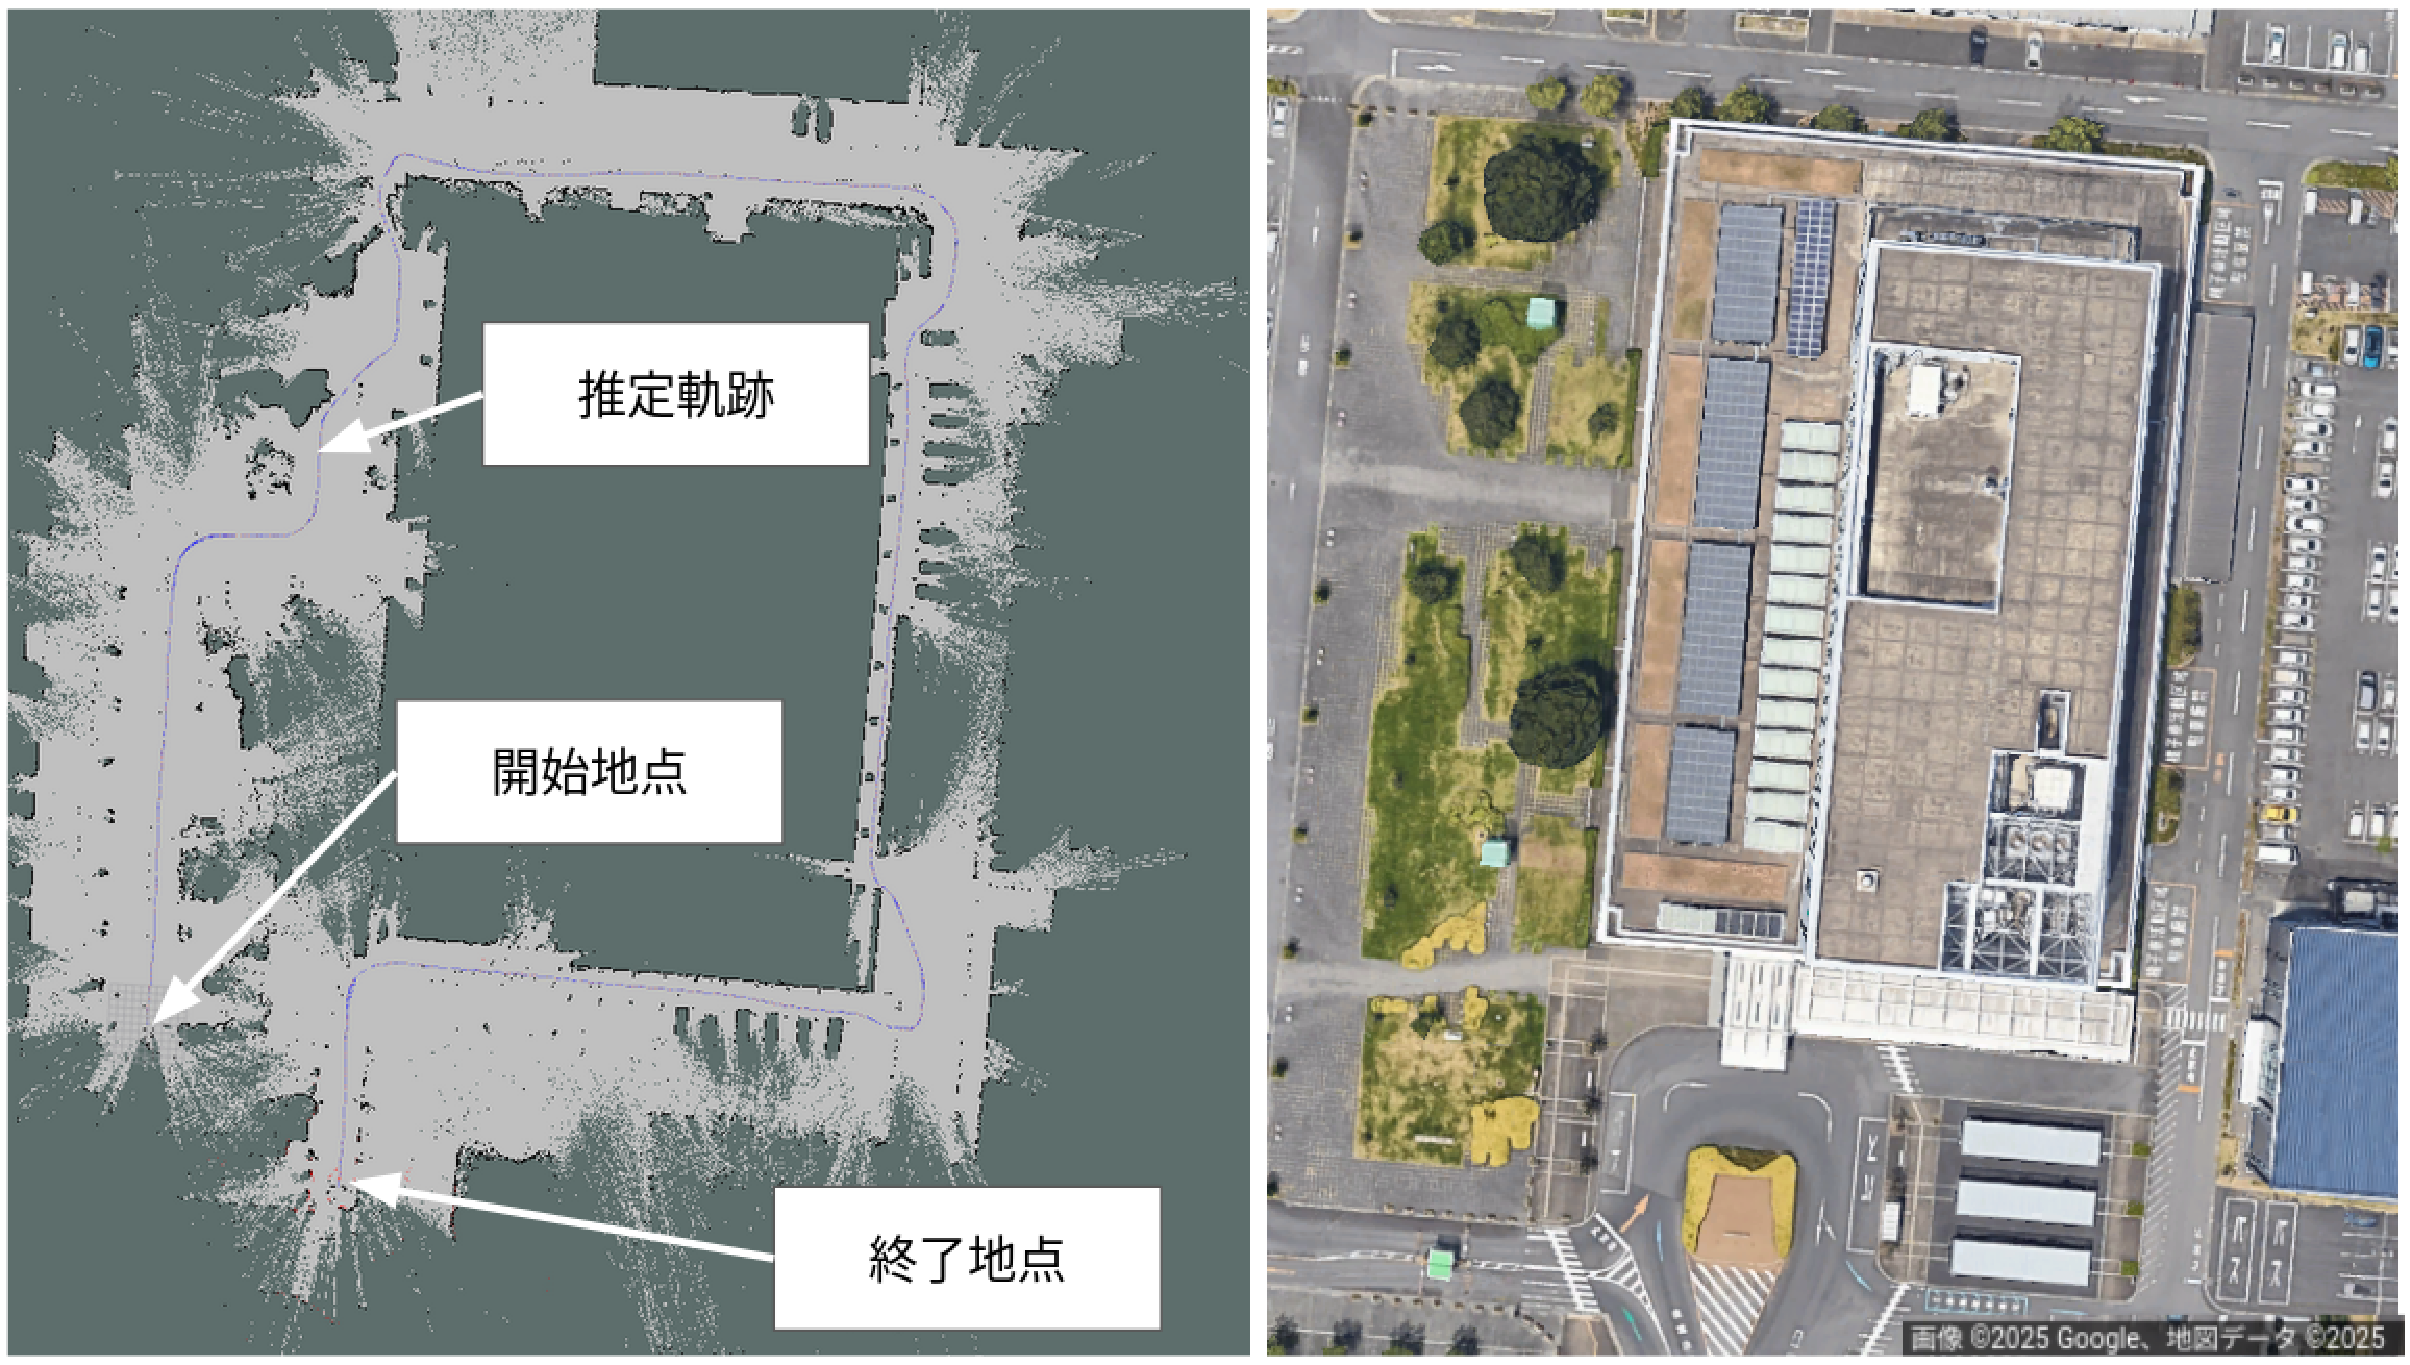
\includegraphics[width=1.0\linewidth]{figs/map.pdf}
    \caption{左: slam\_toolboxで作成した歪みが小さい地図、右: 実環境}
    \label{fig:map}
  \end{center}
\end{figure}

\paragraph{確認走行区間を完走}
確認走行区間の完走については、技術的課題に直面する場面があり、目標は達成したものの苦戦した。
苦労した点については  \ref{sec:4} 節で詳述するが、自己位置推定 に関連するものである。
自己位置推定の問題に対処した後は、確認走行区間の完走という目標のハードルが大幅に下がった。

\subsection{本走行・実験走行で見つかった課題}\label{sec:4}

本チームは、10/6、10/26-27、11/9-10、11/25、12/6-7-8の
計 9 日間にわたり、実験走行および本走行に参加した。
これらの走行で見つかった課題を以下に挙げる。

\paragraph{地図と実際の環境との違い}
実験走行において、スタート地点付近で自己位置がロストする課題が発生した。
この原因は、地図と実際の環境(センシング結果)との間に整合性がないことに起因する。

この影響により、パーティクルの分布が広がったものの、真の位置をカバーするパーティクルが不足していた。
その結果、一部のパーティクルが誤った位置で高い重みを持ち、自己位置推定が局所解に陥ったと考えられる。

対策として、パーティクルの予測・観測更新頻度を増加させることで、真の位置周辺にパーティクルが配置される確率を高める方法を採用した。
その対応として、nav2\_amcl の以下のパラメータを調整した。

\begin{itemize}
  \item \texttt{update\_min\_a[rad]}: 0.2 から 0.1 に変更  
  \item \texttt{update\_min\_d[m]}: 0.25 から 0.125 に変更  
\end{itemize}
これにより観測更新頻度が高まり、自己位置ロストの問題に対応した。

% \paragraph{グローバルプランナーの経路選択}
% 本チームが使用したグローバルプランナーは、地図上にある障害物や侵入可能領域外との境界からできるだけ離れたルートを選択する。
% これにより、市役所裏側の道路では障害物が少ないため、道路の中心を走行してしまうという課題があった。
% この課題は地図上の侵入可能領域を狭くし、道路の端しか通ることができないようにすることで解消したが、
% 侵入可能領域を狭くすることは自己位置ロストのしやすさとトレードオフの関係にある。
% そのため、今後はグローバルプランナーの調整により障害物からできるだけ離れるような
% 経路選択を行わせないようにすべきであると考えられる。

\paragraph{地図作成時における推定旋回量のずれ}
確認走行区間を超えた先の地図作成において、ロボットの推定旋回量にずれが生じる課題が発生した。
この課題は、Yaw方向の姿勢推定誤差が大きいことが主な要因と考えられる。
現時点では解消できていないが、カルマンフィルタを用いてIMUの情報を統合し、Yaw方向の推定精度を向上させることで解消できると考えられる。

\paragraph{3次元点群の抽出高さ}
実験走行において、車止めを検知できずに衝突する課題が発生した。
この問題は、3 次元点群を 2 次元に変換する歳の高さパラメータを適切に調整することで解消した。

しかし、抽出高さを低く設定すると、地面の傾斜や起伏の影響を受けやすくなり、遠方の地面を障害物と誤認するリスクが高まる。
そのため、今後は地面と障害物を適切に識別するロジックを導入し、この問題を解消する必要がある。

\section{その他の試み: スマートフォンを使用した信号認識}

\subsection{課題選択}
本章では、つくばチャレンジの選択課題B「信号認識横断」に向けた取り組みについて述べる。
本チームは、今年度の目標として確認走行区間の完遂を掲げていたが、将来的な発展を視野に入れ、信号認識の技術検証を並行して進めた。
特に、ロボット本体を必要とせずデータ収集およびアルゴリズムの開発を実施できる点を考慮し、本課題を選択した。

\subsection{ハードウェア選定}
本課題では、日の当たり方が大きく異なる信号をミスなくかつ素早く検出することが求められる。
そのためカメラはホワイトバランス調整などが行えるものであり、
加えて、チームの目的も踏まえると安価であることが好ましい。
そこで、スマートフォンをカメラとして採用した。
一般的なスマートフォンには上記の機能が備わっており、旧型モデルを使用することでコストも抑えられる。
本チームでは図\ref{fig:smartphone}に示す2020年発売のGalaxy A21 SCV49を採用した。
2025年1月現在、市場価格で1万円前後である。

\subsection{信号認識手法}
本課題を達成するためには、歩行者用信号(以下、信号)の検出および、横断歩道内で停止している自動車の有無の確認など、安全確認が求められる。
そこで、本チームは深層学習による物体認識手法を用いた。
物体認識に用いる学習済みモデルは、VIDVIP\cite{BabaVIDVIP}が提供している,vidvipo\_yolov8nとした。
認識結果の例を図\ref{fig:result_yolo}に示す。
本モデルは交通環境下での物体認識に特化しており、以下の特性を有する。

\begin{itemize}
    \item 信号や車両、横断歩道などの高精度な認識が可能
    \item 追加学習なしで実用レベルの認識精度を達成
    \item YOLOv8ベースのため、従来手法と比較して処理速度が高速
\end{itemize}

\subsection{信号認識の結果}
事前に取得した課題コース上の動画を本モデルに認識させたところ、青信号が検出できない場合があることを確認した。
% これは、\textbf{@@ここに理由を記載してほしい 海老田へ@@}という可能性がある。
これは、青信号と背景の空の色合いが似通っていたからという可能性がある。

この問題に対処するため、赤信号の検出には YOLOv8 を用い、青信号の検出には画像処理を組み合わせたハイブリッド手法を導入した。
具体的には、信号機の上部(赤色領域)と下部(青色領域)の輝度差を利用し、閾値ベースの手法により青信号の検出精度を向上させた。

\subsection{今後の展望}
今年度は、信号の動画を取得し、取得した動画を用いて GPU を搭載したノートパソコン上で本モデルの動作確認を行った。
来年度では実機への搭載を目指し、電力消費量の少なくなるように手法の軽量化を行うとともに、多様な環境での安定した認識などの課題解決に取り組む予定である。
また、スマートフォンのディスプレイを活用し、ロボットの状態表示や一時停止の解除機能も合わせて開発を行いたい。

\begin{figure}[h]
  \begin{center}
    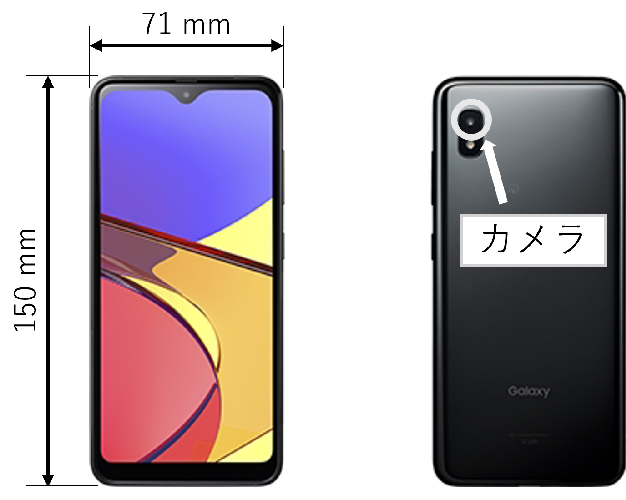
\includegraphics[width=0.6\linewidth]{figs/smartphone.pdf}
    \caption{使用したカメラ(スマートフォン)の外観}
    \label{fig:smartphone}
  \end{center}
\end{figure}

\begin{figure}[h]
  \begin{center}
    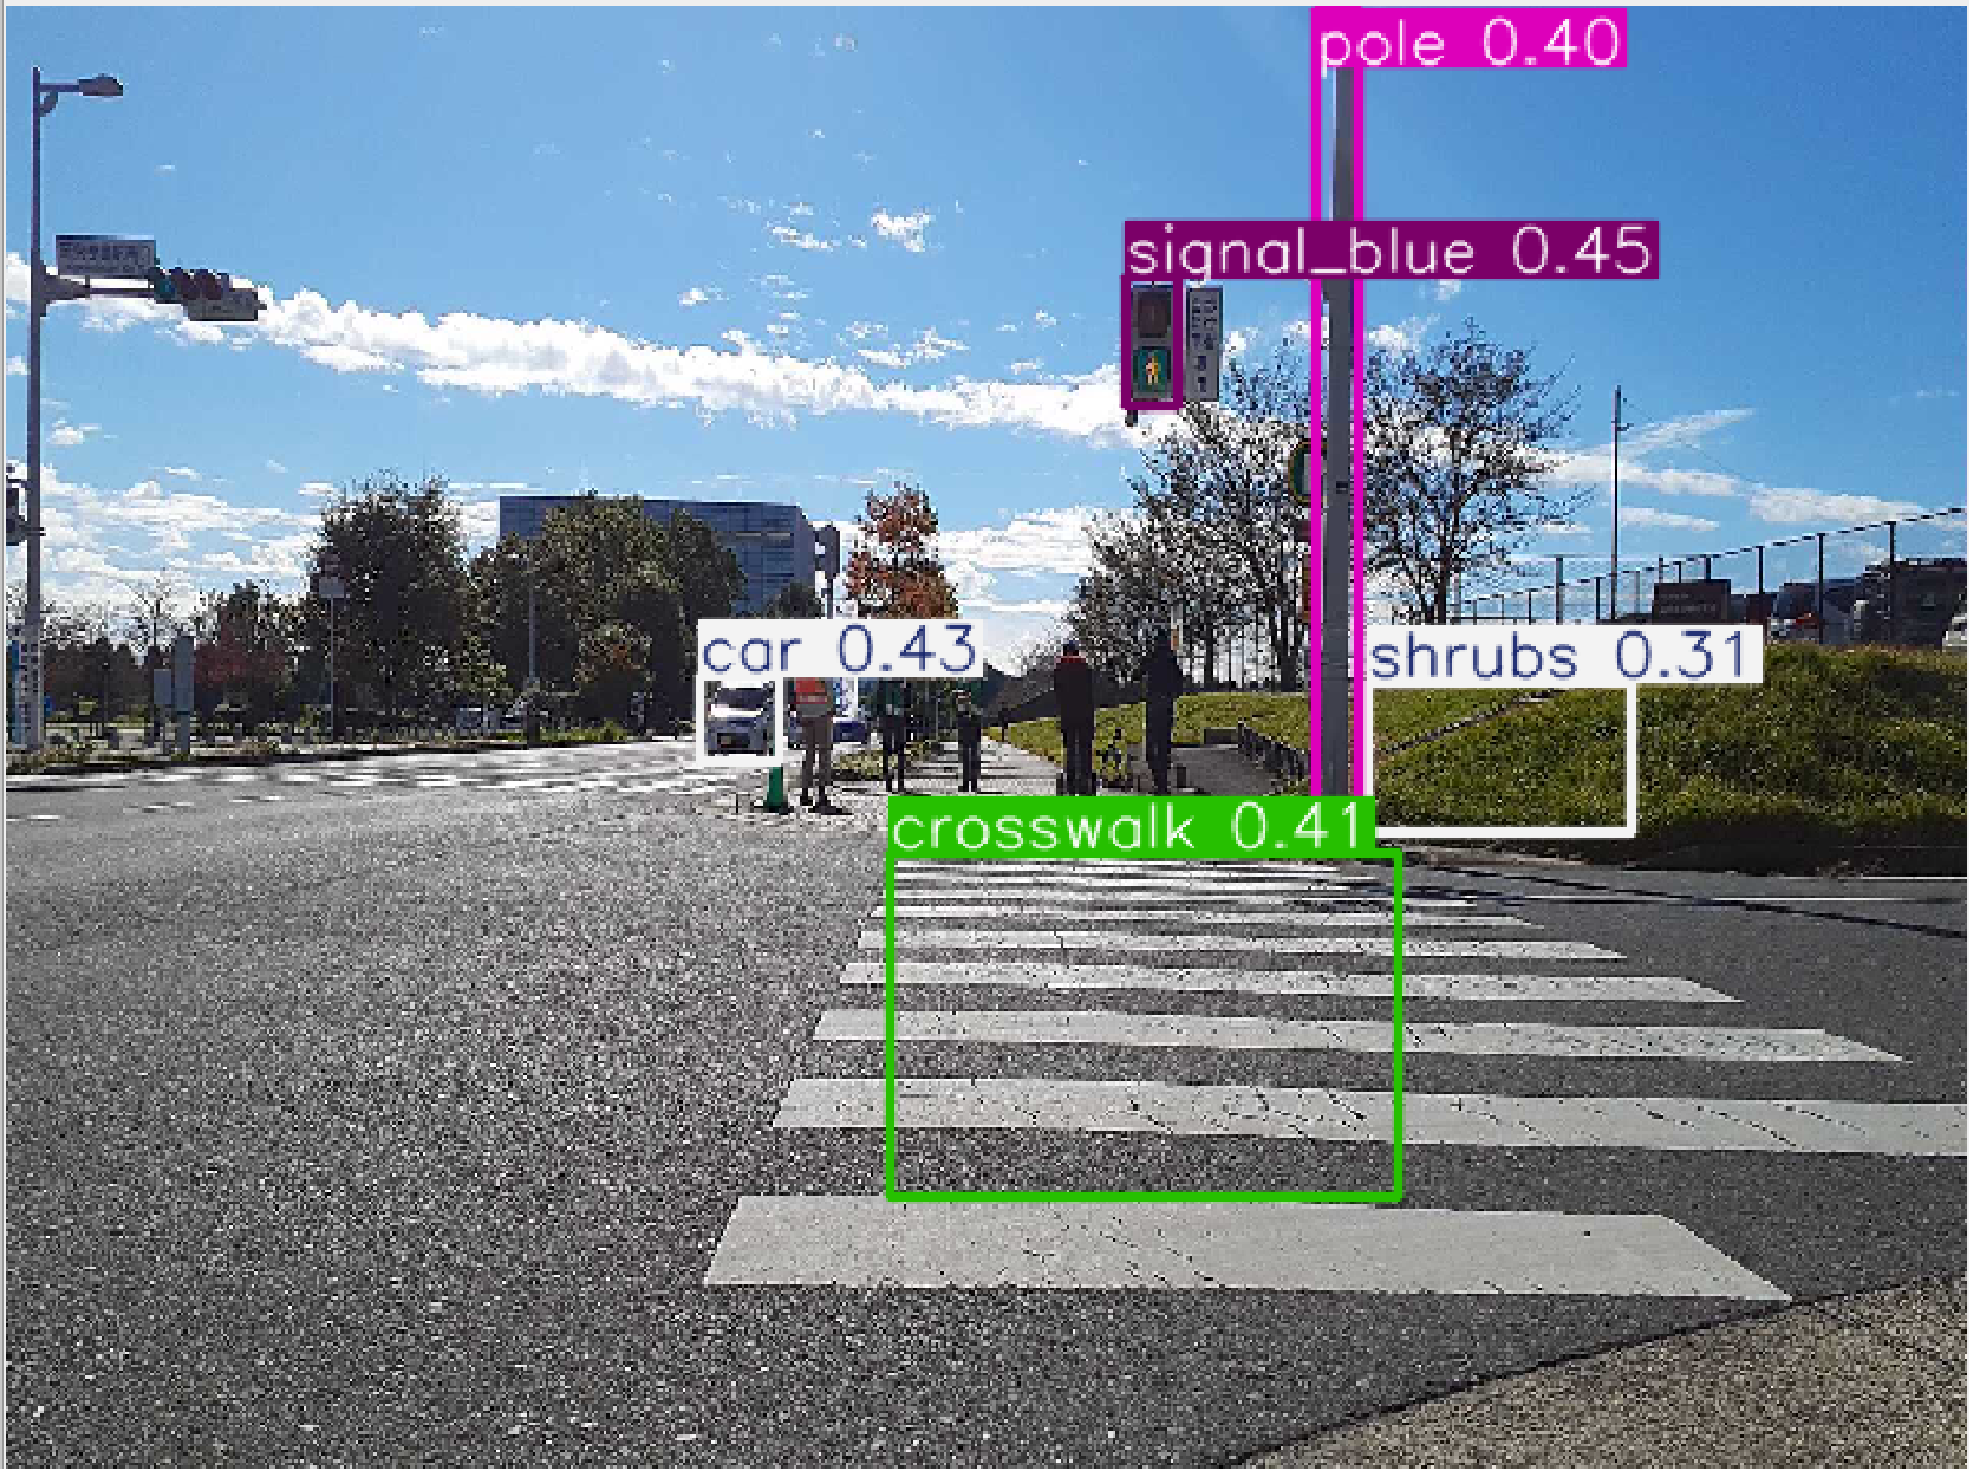
\includegraphics[width=1.0\linewidth]{figs/result_of_yolo.pdf}
    \caption{VIDVIP提供モデルによる認識の例}
    \label{fig:result_yolo}
  \end{center}
\end{figure}
% \newpage
\section{結言}
本チームは今後、新卒でつくばチャレンジに参加するチームが増えることを目標につくばチャレンジに参加した。
チームメンバーは、つくばチャレンジ経験者から初参加のメンバーまで多様であったが、
ハードウェアおよびソフトウェアの開発を分担し、協力して取り組んだ。
その結果、図 \ref{fig:nakama} に示すように、
チームメンバー全員が集まり、本走行を無事に終えることができ、チームの目標を達成した。

来年度は、今年度の開発内容をもとに、見つかった課題への対策を講じるとともに、
今回開発が間に合わなかった機能を追加し、今回作成したロボットによるコースの完走を目指す。

\begin{figure}[h]
  \begin{center}
    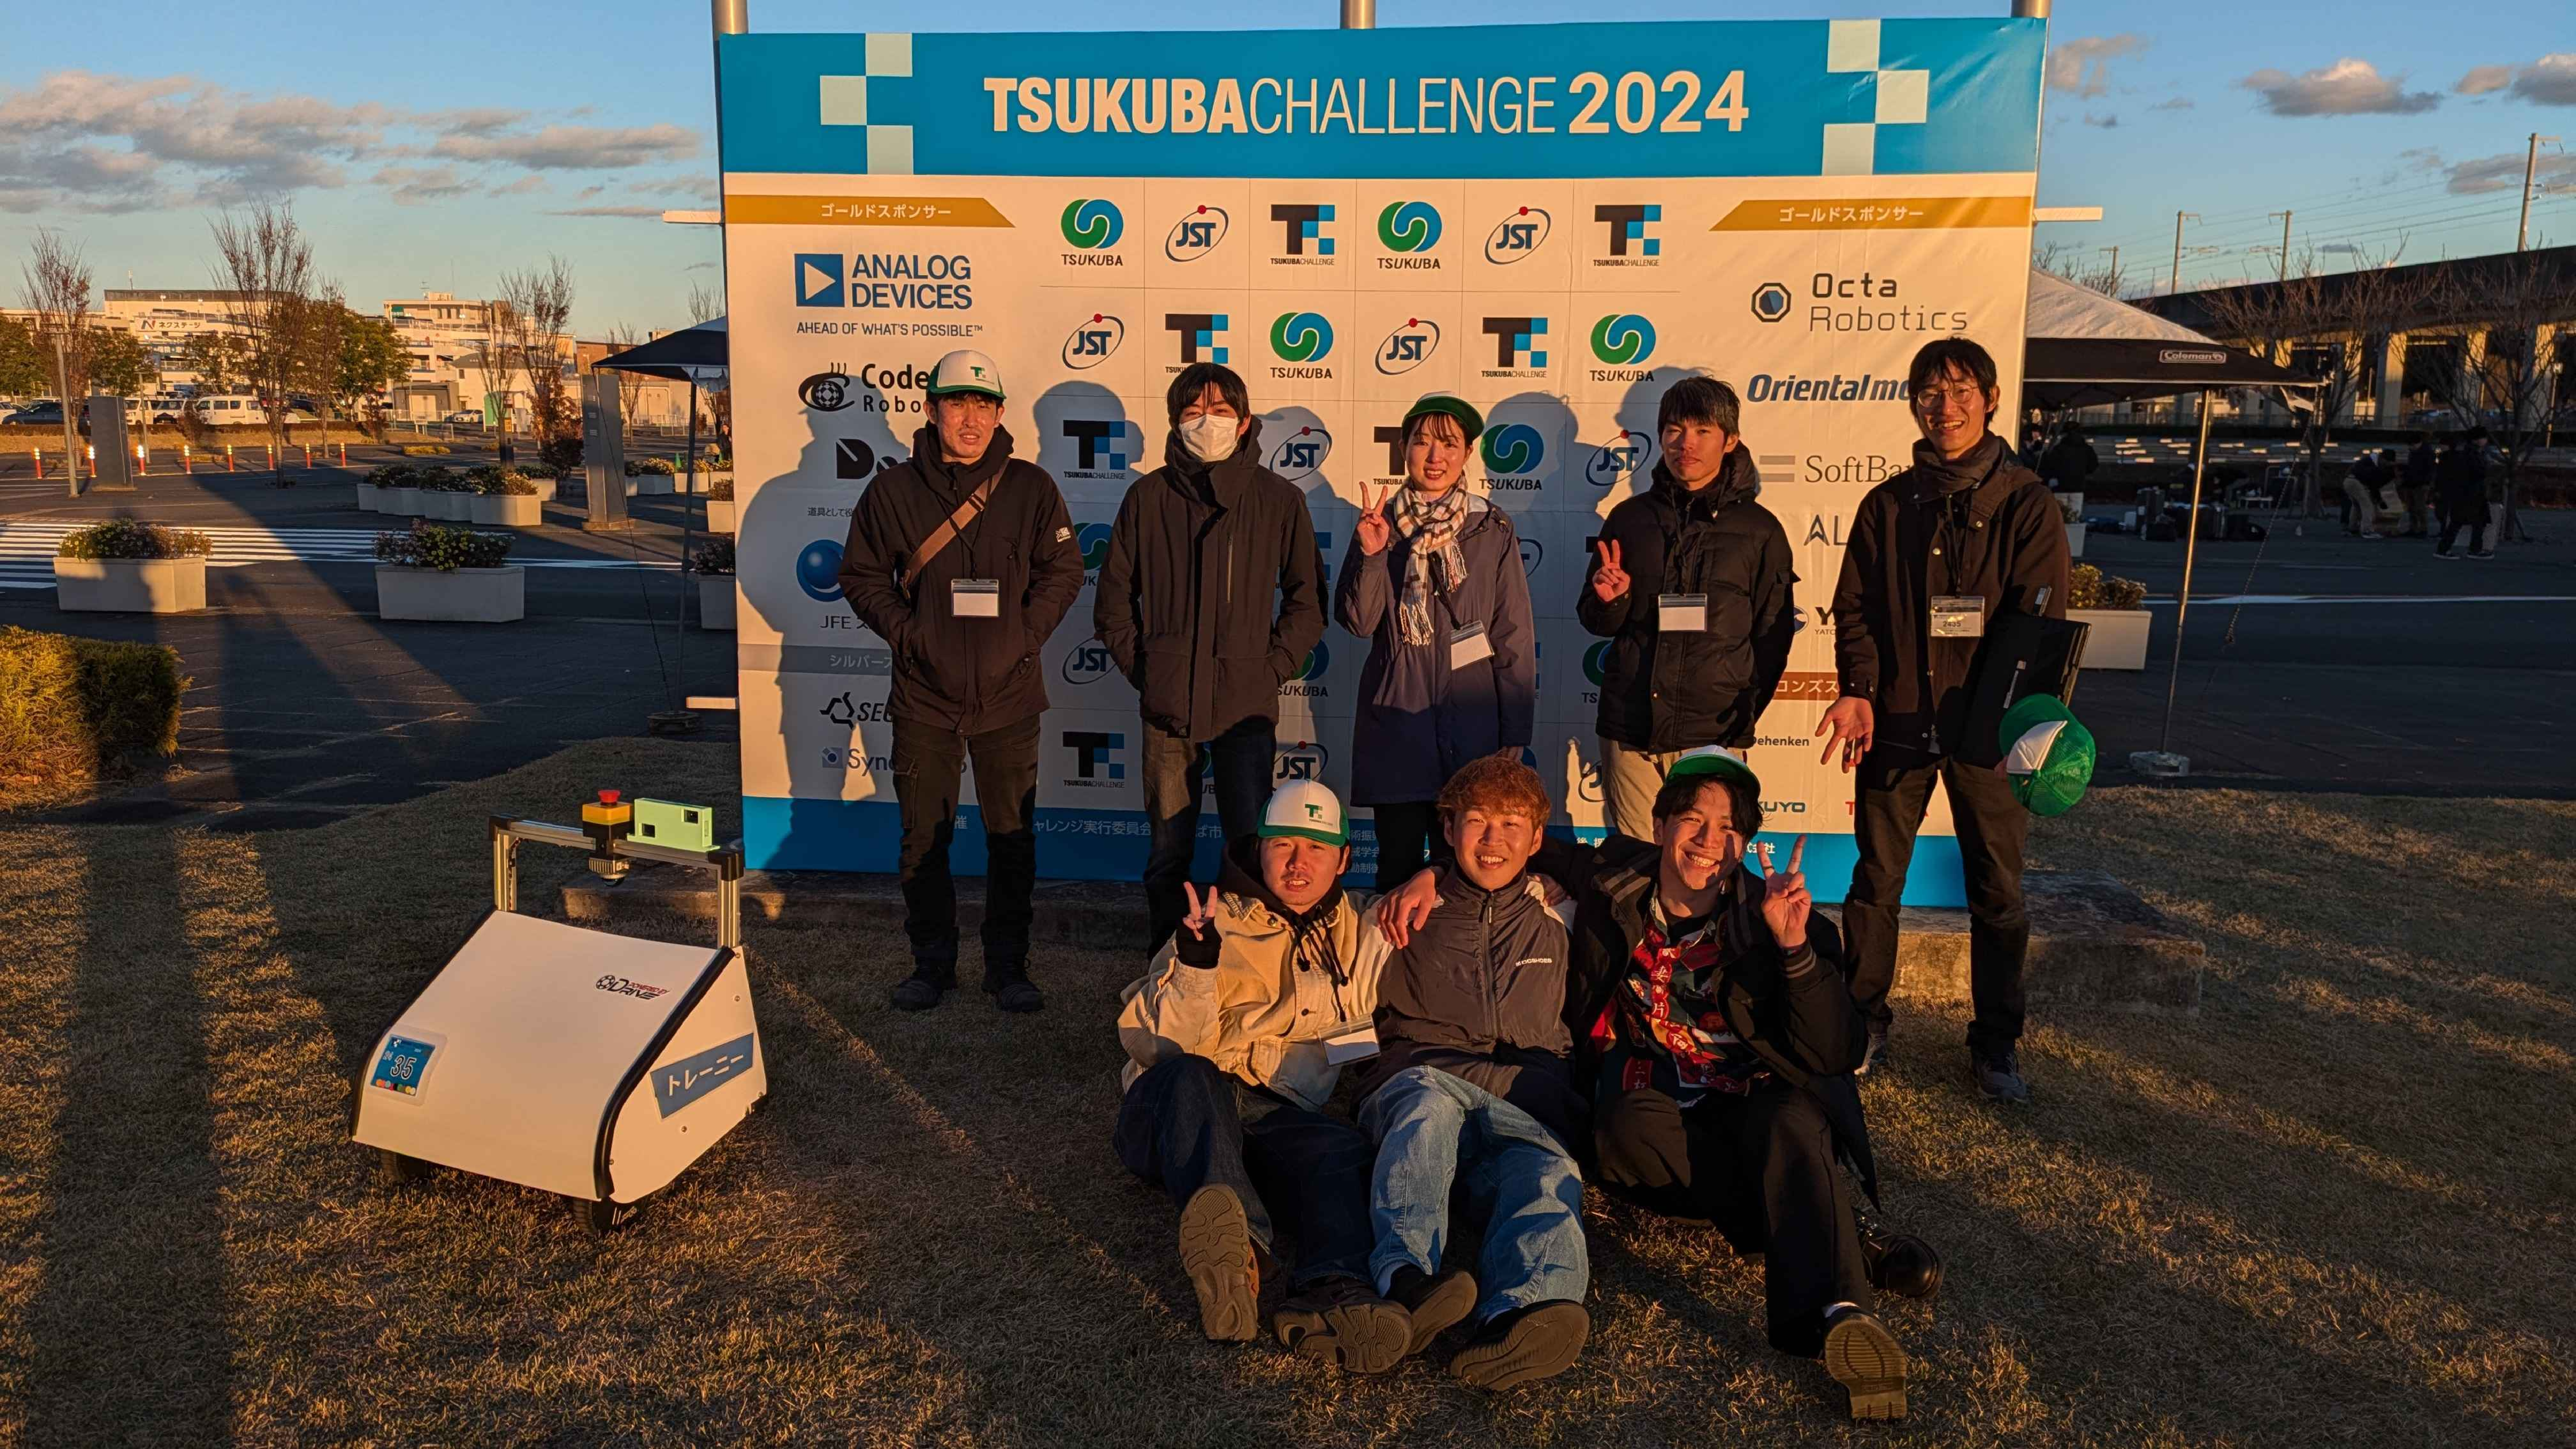
\includegraphics[width=1.0\linewidth]{figs/nakama.pdf}
    \caption{新卒だけどつくばチャレンジ出るよチームのメンバーたち(本走行終了後に撮影)}
    \label{fig:nakama}
  \end{center}
\end{figure}

\section*{謝辞}
つくばチャレンジ実行委員会,つくば市の皆様に感謝申し上げます.
また千葉工大上田研究室,千葉大学の皆様には,つくばチャレンジ2024の参加にあたり、物品の貸与などでご協力頂き感謝申し上げます.

% 参考文献
\footnotesize
\begin{thebibliography}{99}
  \bibitem{ROS 2}
  Macenski, Steven {\it et al.}: ``Robot Operating System 2: Design, architecture, and uses in the wild,''
  Science Robotics, Vol. 7、No. 66, 2022.
  \bibitem{odrive}
  ODrive,BotWheelExplorerKit:\url{https://odriverobotics.com/shop/botwheel-explorer?srsltid=AfmBOorKkTnYnmd8YJIK3zfWzGe1yAGRSF4SxKkbpshUTGtWI_a2NNef}

  \bibitem{PE960_1}
  モノタロウ: ``ポリプレート'',\url{https://www.monotaro.com/p/3576/7697/?} (last visit 2025-01-05)

  % \bibitem{ROS}
  % Morgan Quigley {\it et al.}: ``ROS: an open-source Robot Operating System,''
  % Open-Source Software workshop of the International Conference on Robotics and Automation、2009.
  
  \bibitem{Fusion360}
  Autodesk,\url{https://www.autodesk.com/jp/products/fusion-360/overview?term=1-YEAR&tab=subscription#top} (last visit 2025-01-31)
  
  \bibitem{Onshape}
  PTC,\url{https://www.onshape.com/en/} (last visit 2025-01-31)
  
  \bibitem{mid360}
  Livox Mid-360,\url{https://www.livoxtech.com/jp/mid-360}
  
  \bibitem{nav2_docs}
  Nav2 — Nav2 1.0.0 documentation, \url{https://docs.nav2.org/} (last visit: 2025-01-31).
  
  \bibitem{pcl_lsc}
  ROS Perception: ``ROS Perception/pointcloud\_to\_laserscan (humble branch),'' \url{https://github.com/ros-perception/pointcloud_to_laserscan} (last visit: 2025-01-31).
  
  \bibitem{nav2_amcl}
  ROS2 AMCL: ``navigation2/nav2\_amcl,'' \url{https://github.com/ros-navigation/navigation2/tree/main/nav2_amcl}  (last visit: 2025-01-31).
  
  \bibitem{nav2}
  ROS Navigation: ``ros-navigation/navigation2 (humble branch),'' \url{https://github.com/ros-navigation/navigation2} (last visit: 2025-01-30).
  
  \bibitem{slam_toolbox}
  Steve Macenski: ``slam\_toolbox (ros2 branch),'' \url{https://github.com/SteveMacenski/slam_toolbox} (last visit: 2025-01-31).

  \bibitem{youtube_real_run}
  新卒だけどつくばチャレンジ出るよ つくばチャレンジ2024 本走行(2024/12/8),\url{https://www.youtube.com/watch?v=fuvcGf8-x7I} (last visit 2025-01-31)
  
  \bibitem{BabaVIDVIP}
  T. Baba, “VIDVIP: Dataset for Object Detection During Sidewalk Travel,” J. Robot. Mechatron., Vol.33 No.5, pp. 1135-1143, 2021. https://doi.org/10.20965/jrm.2021.p1135
  
\end{thebibliography}
\normalsize

\clearpage
\end{document}
